\documentclass[12pt,a4paper]{article}
\usepackage[utf8]{inputenc}
\usepackage[french]{babel}
\usepackage[T1]{fontenc}
\usepackage{amsmath, amssymb}
\usepackage{graphicx}
\usepackage{hyperref}
\usepackage{geometry}
\geometry{margin=2.5cm}
\usepackage{float}
\usepackage{xcolor}
\usepackage{booktabs}
\usepackage{listings}
\usepackage{caption}
\usepackage{array}
\usepackage{tabularx}
\usepackage{multirow}
\usepackage{enumitem}

\hypersetup{
    colorlinks=true,
    linkcolor=blue,
    filecolor=magenta,
    urlcolor=cyan,
    pdftitle={Rapport de Projet - Implémentation et Analyse du Chiffrement Solitaire},
    pdfauthor={Yani Mohellebi},
}

\lstset{
    language=Python,
    basicstyle=\ttfamily\small,
    keywordstyle=\color{blue},
    stringstyle=\color{red},
    commentstyle=\color{green!60!black},
    breaklines=true,
    showstringspaces=false,
    frame=single,
    backgroundcolor=\color{gray!10},
    numbers=left,
    numberstyle=\tiny\color{gray},
    stepnumber=1,
    numbersep=8pt,
}

\begin{document}

% ─────────────────────────────────────────────────────────────────────────────
%  PAGE DE TITRE
% ─────────────────────────────────────────────────────────────────────────────
\begin{titlepage}
    \centering
    \vspace*{1.5cm}

    {\scshape\Large Rapport de Projet Universitaire \par}
    \vspace{0.4cm}
    {\large Module : Cryptographie — Master 1 Informatique \par}
    \vspace{1.5cm}

    \rule{\linewidth}{0.5pt}\\[0.4cm]
    {\huge\bfseries Implémentation, Étude et Analyse Sécuritaire\\[0.3cm]
    du Chiffrement Solitaire (Pontifex)\par}
    \rule{\linewidth}{0.5pt}\\[2cm]

    {\Large\itshape Yani Mohellebi\par}
    \vspace{0.5cm}
    {\large Master 1 Informatique\par}
    \vspace{0.3cm}
    {\normalsize \texttt{yanimohellebi@gmail.com}\par}

    \vfill

    \begin{tabular}{rl}
        \textbf{Algorithme étudié :} & Solitaire (Pontifex) — Bruce Schneier, 1999 \\
        \textbf{Technologies :} & Python 3.12, Streamlit, ChromaDB, Gemini API \\
        \textbf{Tests :} & 115/115 validés \\
        \textbf{Année :} & 2025--2026 \\
    \end{tabular}
\end{titlepage}

% ─────────────────────────────────────────────────────────────────────────────
%  TABLES
% ─────────────────────────────────────────────────────────────────────────────
\newpage
\tableofcontents
\newpage
\listoffigures
\newpage

% ─────────────────────────────────────────────────────────────────────────────
%  RÉSUMÉ
% ─────────────────────────────────────────────────────────────────────────────
\begin{abstract}
Ce projet s'inscrit dans le cadre du module de Cryptographie de Master 1. Il consiste en l'étude approfondie, l'implémentation stricte et l'analyse statistique du chiffrement par flux \textit{Solitaire} (ou \textit{Pontifex}), conçu par Bruce Schneier en 1999 pour le roman \textit{Cryptonomicon} de Neal Stephenson. L'espace de clés théorique est colossal ($54! \approx 2{,}31 \times 10^{71} \approx 2^{237}$ permutations), mais nos expériences statistiques révèlent un biais structurel mesurable découvert par Paul Crowley : la probabilité de répétition entre deux valeurs consécutives du flux est $1/22{,}5$ au lieu de l'idéal $1/26$. Sur un échantillon de 2\,000 valeurs, nous mesurons une entropie de Shannon $H(X) \approx 4{,}693$ bits (pour un maximum théorique de $4{,}700$ bits) et un indice de coïncidence $\text{IC} \approx 0{,}03839$, confirmant quantitativement ce biais. L'application développée en Python et propulsée par Streamlit intègre trois composantes d'Intelligence Artificielle : un assistant RAG (ChromaDB + Gemini 2.5 Flash), un pipeline de génération des 54 visuels de cartes (Gemini Image + Pillow), et un module d'interprétation analytique (Gemini 2.5 Pro). La suite de 115 tests automatisés valide l'exactitude de l'implémentation, incluant les trois vecteurs officiels de Schneier. Ces résultats confirment que si Solitaire ne satisfait pas aux exigences d'un chiffrement moderne, il conserve une valeur pédagogique exceptionnelle pour l'étude des générateurs pseudo-aléatoires à état interne évolutif.
\end{abstract}

% ─────────────────────────────────────────────────────────────────────────────
%  1. INTRODUCTION
% ─────────────────────────────────────────────────────────────────────────────
\section{Introduction}

\subsection{Contexte}
Dans son roman \textit{Cryptonomicon} paru en 1999, l'auteur Neal Stephenson met en scène des personnages devant communiquer secrètement sans éveiller les soupçons, c'est-à-dire sans avoir recours à du matériel informatique ou des outils cryptographiques évidents. Il a sollicité l'expert en cryptographie Bruce Schneier pour concevoir un algorithme réaliste répondant à cette contrainte. Le résultat est le chiffrement \textbf{Solitaire}, un algorithme par flux (\textit{stream cipher}) capable de fournir une sécurité importante tout en étant exécutable à la main avec un simple jeu de 54 cartes (52 cartes classiques et 2 jokers). Dans le roman, Schneier le désigne sous le pseudonyme \textit{Pontifex} afin de le dissimuler.

\subsection{Problématique et Objectifs}
L'enjeu de ce projet est multiple. Il s'agit tout d'abord de comprendre comment une simple permutation physique d'un jeu de cartes peut modéliser un Générateur de Nombres Pseudo-Aléatoires Cryptographiquement Sécurisé (CPRNG). Ensuite, le défi technique consiste à transposer cet algorithme hautement manuel en une application informatique robuste, visuellement didactique et architecturée selon les normes académiques.

Nos objectifs sont :
\begin{enumerate}[label=\textbf{O\arabic*.}]
    \item Implémenter strictement l'algorithme en respectant les vecteurs de tests officiels de Schneier, y compris tous les cas limites de déplacement des jokers.
    \item Offrir une interface utilisateur permettant de visualiser chaque étape de transformation du paquet, incluant un moteur de démonstration animé.
    \item Évaluer empiriquement la robustesse de l'algorithme à l'aide de tests statistiques rigoureux (χ², entropie de Shannon, IC, test des runs NIST SP 800-22).
    \item Documenter et démontrer les vulnérabilités connues : biais de Crowley et attaque par réutilisation de clé (\textit{crib-dragging}).
    \item Intégrer trois composantes d'Intelligence Artificielle : assistant RAG, génération visuelle par IA, et interprétation analytique automatique.
\end{enumerate}

% ─────────────────────────────────────────────────────────────────────────────
%  2. ÉTAT DE L'ART ET CONTEXTE THÉORIQUE
% ─────────────────────────────────────────────────────────────────────────────
\section{État de l'art et Contexte Théorique}

\subsection{Le Chiffrement par Flux (Stream Cipher)}
Contrairement aux algorithmes par blocs (comme AES ou DES) qui chiffrent des portions fixes de données, un chiffrement par flux combine le texte clair avec un flux de clés (\textit{keystream}) pseudo-aléatoire généré en continu, généralement via une opération XOR ou, dans le cas du Solitaire, par une addition modulaire modulo 26.

L'opération de chiffrement pour un caractère clair $P_i$ et une valeur de flux $K_i$ s'écrit :
\begin{equation}
C_i = \begin{cases} (P_i + K_i) \bmod 26 & \text{si } (P_i + K_i) \not\equiv 0 \pmod{26} \\ 26 & \text{sinon (lettre Z)} \end{cases}
\end{equation}
Le déchiffrement s'effectue par l'opération inverse :
\begin{equation}
P_i = \begin{cases} (C_i - K_i) \bmod 26 & \text{si } (C_i - K_i) > 0 \\ (C_i - K_i) + 26 & \text{sinon} \end{cases}
\end{equation}
La convention $0 \equiv 26$ (la lettre Z, et non A) est une source fréquente d'erreur d'implémentation.

\subsection{Notations et Système de Valeurs Bridge}
L'algorithme Solitaire utilise deux systèmes de valeurs distincts qu'il convient de ne pas confondre :

\begin{table}[H]
\centering
\caption{Correspondance entre valeurs Bridge et valeurs de chiffrement}
\begin{tabular}{lcc}
\toprule
\textbf{Carte} & \textbf{Valeur Bridge} & \textbf{Valeur chiffrement} \\
\midrule
As de Trèfle & 1 & 1 \\
Roi de Trèfle & 13 & 13 \\
As de Carreau & 14 & 14 \\
\ldots & \ldots & \ldots \\
Roi de Pique & 52 & 26 \\
Joker A (noir) & 53 & ignoré (joker) \\
Joker B (rouge) & 54 & ignoré (joker) \\
\bottomrule
\end{tabular}
\label{tab:valeurs_bridge}
\end{table}

La valeur Bridge est utilisée aux opérations 4 et 5 (coupes et lecture de sortie). Les deux jokers valent 53 en valeur Bridge pour l'opération 4. La valeur de chiffrement ($v \bmod 26$, avec $0 \to 26$) est uniquement produite à l'étape 5 et ne concerne jamais les jokers.

\subsection{L'Algorithme Solitaire — Formalisation}
L'état interne du générateur est une permutation $S_t \in \mathcal{S}_{54}$ du paquet. La génération d'une valeur du flux nécessite cinq étapes consécutives sur cet état :

\begin{enumerate}
    \item \textbf{Avancée du Joker A} : Le Joker A (valeur Bridge 53) est descendu d'une position (échange avec la carte suivante). \textit{Cas limite :} si A est en dernière position, il passe en deuxième position — jamais en première.

    \item \textbf{Avancée du Joker B} : Le Joker B (valeur Bridge 54) est descendu de deux positions. \textit{Cas limites :} si B est en avant-dernière, il passe en 2\ieme{} ; en dernière, il passe en 3\ieme{}. Le Joker B ne peut jamais être en première position.

    \item \textbf{Triple Coupe} : Les deux jokers divisent le paquet en trois segments $\langle \text{Haut}, \text{Milieu (jokers inclus)}, \text{Bas} \rangle$. L'opération échange Haut et Bas ; le segment central reste fixe.
    \begin{equation*}
        S \leftarrow \text{Bas} \oplus \text{Milieu} \oplus \text{Haut}
    \end{equation*}
    Si un joker est en première ou dernière position, l'un des segments est vide — cas valide.

    \item \textbf{Coupe Simple (Counted Cut)} : Soit $v$ la valeur Bridge de la \textbf{dernière} carte (1 à 53 pour les jokers). On prend les $v$ premières cartes et on les insère juste avant la dernière carte, qui \textbf{ne bouge jamais}.

    \item \textbf{Lecture de la Sortie} : Soit $n$ la valeur Bridge de la \textbf{première} carte. La carte en position $n+1$ produit la sortie. Si c'est un joker : ignorer et recommencer en 1. Sinon : $K_i = \left((n+1) \bmod 26\right)$, avec $0 \to 26$.
\end{enumerate}

\subsection{Comparaison des Stream Ciphers}

\begin{table}[H]
\centering
\caption{Comparaison de Solitaire avec les principaux algorithmes par flux}
\begin{tabularx}{\textwidth}{lXXXX}
\toprule
\textbf{Critère} & \textbf{Solitaire} & \textbf{RC4} & \textbf{ChaCha20} & \textbf{AES-CTR} \\
\midrule
Type & Stream cipher & Stream cipher & Stream cipher & Block (mode CTR) \\
Taille de l'état & 54 cartes & 256 octets & 512 bits & 128 bits \\
Espace de clés & $\approx 2^{237}$ & $2^{128}$ & $2^{256}$ & $2^{128}$--$2^{256}$ \\
Biais statistique & Oui (Crowley) & Oui (premiers octets) & Non & Non \\
Authentification & Non & Non & Oui (Poly1305) & Non \\
Exécutable à la main & \textbf{Oui} & Non & Non & Non \\
Standard actuel & Non (pédagogique) & Non (RFC 7465) & Oui (RFC 8439) & Oui \\
\bottomrule
\end{tabularx}
\label{tab:comparaison_ciphers}
\end{table}

% ─────────────────────────────────────────────────────────────────────────────
%  3. CONCEPTION ET ARCHITECTURE TECHNIQUE
% ─────────────────────────────────────────────────────────────────────────────
\section{Conception et Architecture Technique}

\subsection{Architecture Globale en Couches}
Le projet suit une séparation stricte des préoccupations (Architecture en couches / principe de responsabilité unique) :

\begin{table}[H]
\centering
\caption{Modules du projet et leur rôle}
\begin{tabularx}{\textwidth}{llX}
\toprule
\textbf{Module} & \textbf{Fichiers principaux} & \textbf{Rôle} \\
\midrule
\texttt{core/} & \texttt{deck.py, solitaire.py,} & Noyau algorithmique pur. Fonctions \\
 & \texttt{keystream.py, encryption.py} & immuables, aucune dépendance externe. \\
\addlinespace
\texttt{ui/} & \texttt{app.py, tab\_encrypt.py,} & Interface Streamlit. Gestion de l'état \\
 & \texttt{tab\_demo.py, tab\_analysis.py,} & de session, événements, présentation. \\
 & \texttt{tab\_assistant.py, tab\_rapport.py} & \\
\addlinespace
\texttt{ai/} & \texttt{assistant.py, knowledge/*.txt} & RAG : ChromaDB + Gemini 2.5 Flash. \\
\addlinespace
\texttt{visuals/} & \texttt{card\_loader.py,} & Génération et cache des images. \\
 & \texttt{download\_real\_deck.py} & Pipeline Pillow de post-traitement. \\
\addlinespace
\texttt{security/} & \texttt{key\_reuse\_demo.py,} & Démonstrations d'attaques et tests \\
 & \texttt{crypto\_analysis.py} & statistiques (χ², entropie, IC, runs). \\
\addlinespace
\texttt{tests/} & \texttt{test\_*.py} (8 fichiers) & Suite pytest : 115 tests, 3 catégories. \\
\bottomrule
\end{tabularx}
\label{tab:modules}
\end{table}

\subsection{Environnement Technologique}
Le langage \textbf{Python 3.12} a été retenu pour son expressivité (slicing de tuples, compréhensions), ses puissantes capacités d'analyse (NumPy, SciPy) et son écosystème IA mature (ChromaDB, google-generativeai). Le tableau \ref{tab:techstack} résume la pile technologique complète.

\begin{table}[H]
\centering
\caption{Pile technologique du projet}
\begin{tabular}{lll}
\toprule
\textbf{Domaine} & \textbf{Bibliothèque / Service} & \textbf{Version / Usage} \\
\midrule
Interface web & Streamlit & UI interactive, état de session \\
IA — LLM & Gemini 2.5 Flash / Pro & RAG, interprétation analytique \\
IA — Embeddings & gemini-embedding-001 & Vectorisation des chunks \\
IA — Image & Gemini Image & Génération des 54 cartes \\
Base vectorielle & ChromaDB & Stockage et recherche des chunks \\
Analyse & NumPy, SciPy, Plotly & Tests statistiques, graphiques \\
Image & Pillow & Post-traitement des cartes \\
Tests & pytest & 115 tests automatisés \\
\bottomrule
\end{tabular}
\label{tab:techstack}
\end{table}

% ─────────────────────────────────────────────────────────────────────────────
%  4. RÉALISATION ET IMPLÉMENTATION
% ─────────────────────────────────────────────────────────────────────────────
\section{Réalisation et Implémentation}

\subsection{Représentation Immuable du Paquet}
Pour prévenir les effets de bord, l'état du jeu de cartes a été implémenté à l'aide d'un \texttt{tuple} immuable d'entiers. À chaque étape, une nouvelle copie du tuple est retournée — aucune mutation en place.

Ce choix de conception garantit que :
\begin{itemize}
    \item Chaque opération est une \textbf{fonction pure} : \texttt{(tuple[int, ...]) → tuple[int, ...]}.
    \item Les états intermédiaires du moteur de démonstration peuvent être conservés sans copie défensive.
    \item Les tests unitaires s'écrivent naturellement sans besoin de \textit{fixtures} complexes.
\end{itemize}

Par exemple, l'opération de la Triple Coupe s'écrit de manière concise et sécurisée :
\begin{lstlisting}[language=Python, caption={Implémentation de la Triple Coupe (core/solitaire.py)}]
def triple_cut(deck: tuple[int, ...]) -> tuple[int, ...]:
    idx1, idx2 = sorted([deck.index(53), deck.index(54)])
    top    = deck[:idx1]
    middle = deck[idx1:idx2 + 1]   # jokers inclus
    bottom = deck[idx2 + 1:]
    return bottom + middle + top
\end{lstlisting}

\subsection{Initialisation par Mot de Passe (Keying)}
L'initialisation du paquet à partir d'un mot de passe secret est la procédure qui lie la clé symétrique à l'état initial du générateur. Elle suit la méthode définie par Schneier :

\begin{enumerate}
    \item Partir du paquet dans l'ordre standard : $(1, 2, \ldots, 52, 53, 54)$.
    \item Pour \textbf{chaque lettre} $\ell$ du mot de passe (valeur numérique $v_\ell$, $A=1, \ldots, Z=26$) :
    \begin{enumerate}[label=\alph*.]
        \item Appliquer les opérations 1, 2, 3 et 4 (sans lecture de sortie).
        \item Effectuer une coupe supplémentaire en utilisant $v_\ell$ comme paramètre de coupe.
    \end{enumerate}
\end{enumerate}

\begin{equation}
    S_{\text{init}} = \text{Key}(S_0, \ell_1) \circ \text{Key}(S_1, \ell_2) \circ \cdots \circ \text{Key}(S_{k-1}, \ell_k)
\end{equation}

\begin{lstlisting}[language=Python, caption={Algorithme de keying (core/keystream.py)}]
def key_deck(key: str) -> tuple[int, ...]:
    deck = create_deck()   # (1, 2, ..., 54)
    for char in key.upper():
        if char.isalpha():
            v = ord(char) - ord('A') + 1   # A=1 ... Z=26
            deck = move_joker_a(deck)
            deck = move_joker_b(deck)
            deck = triple_cut(deck)
            deck = count_cut(deck)
            deck = count_cut_with_n(deck, v)  # coupe par la valeur du caractere
    return deck
\end{lstlisting}

Schneier recommande un mot de passe d'au moins 64 à 80 caractères pour une sécurité maximale. En pratique, des mots de passe courts réduisent drastiquement l'espace de clés effectif.

\subsection{Moteur de Démonstration Pédagogique}
L'un des apports majeurs de l'application est le \textbf{moteur de démonstration} (\texttt{ui/demo\_engine.py}), qui pré-calcule l'intégralité des états du paquet pour chaque lettre du message à chiffrer, permettant une navigation interactive pas-à-pas.

Chaque étape est modélisée par une \texttt{dataclass} typée :
\begin{lstlisting}[language=Python, caption={Structure d'une étape de démonstration (ui/demo\_engine.py)}]
@dataclass
class EncryptionStep:
    letter_idx:   int
    plain_char:   str
    op_num:       int | str
    op_name:      str
    deck_before:  tuple[int, ...]
    deck_after:   tuple[int, ...]
    center_cards: list[int]       # cartes mises en valeur
    highlights:   dict[int, str]  # carte -> couleur CSS
    output_val:   int | None = None
    cipher_char:  str = ''
\end{lstlisting}

Ce découpage permet à l'interface Streamlit d'afficher l'état du paquet avant et après chaque opération, avec surbrillance des cartes modifiées, sans recalculer l'algorithme à chaque interaction.

\subsection{Visuels et Interface Utilisateur}
L'interface graphique, de style Cyberpunk, propose trois thèmes d'affichage des cartes :

\begin{itemize}
    \item \textbf{Cyberpunk (sombre)} : 54 PNG générés par l'API Gemini Image, post-traités par \texttt{Pillow} pour ajouter le rang, le symbole de famille et le numéro Bridge.
    \item \textbf{Classique (réaliste)} : photographies de vraies cartes à jouer.
    \item \textbf{Académique (SVG)} : rendu CSS pur, utilisé dans ce rapport pour sa légèreté.
\end{itemize}

\begin{figure}[H]
    \centering
    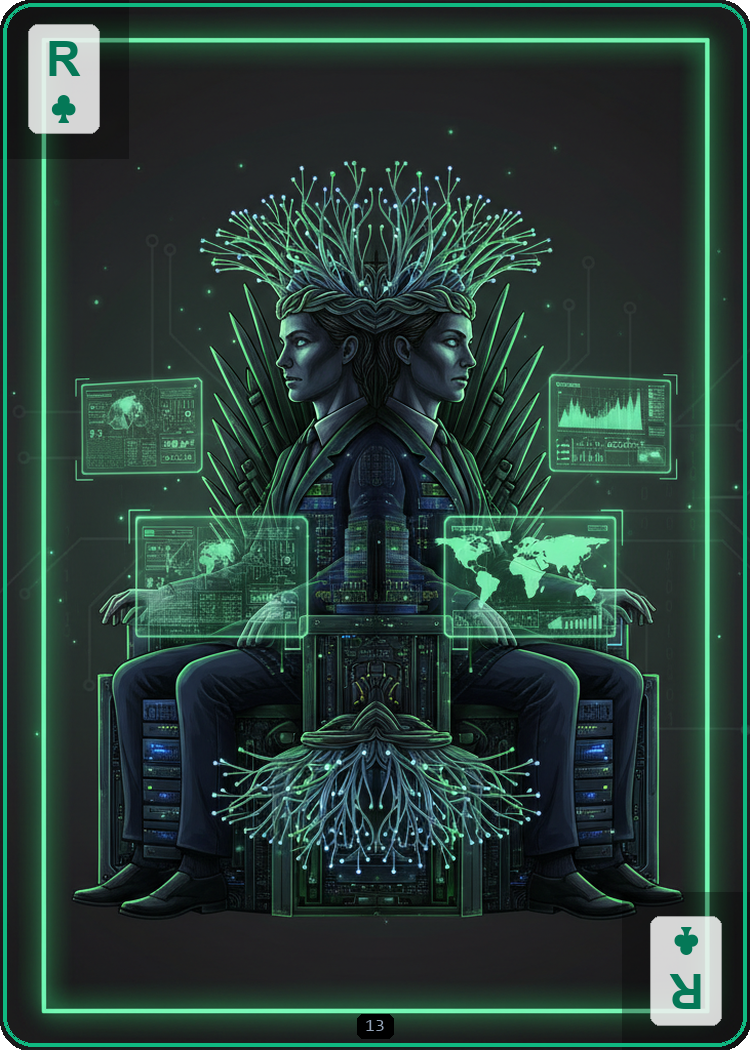
\includegraphics[height=5cm]{rapport_assets/13_king.png}
    \caption{Carte générée par Gemini Image (thème Cyberpunk) : Roi de Trèfle avec post-traitement Pillow (surimpression du rang, du symbole et du numéro Bridge).}
    \label{fig:card_example}
\end{figure}

\begin{figure}[H]
    \centering
    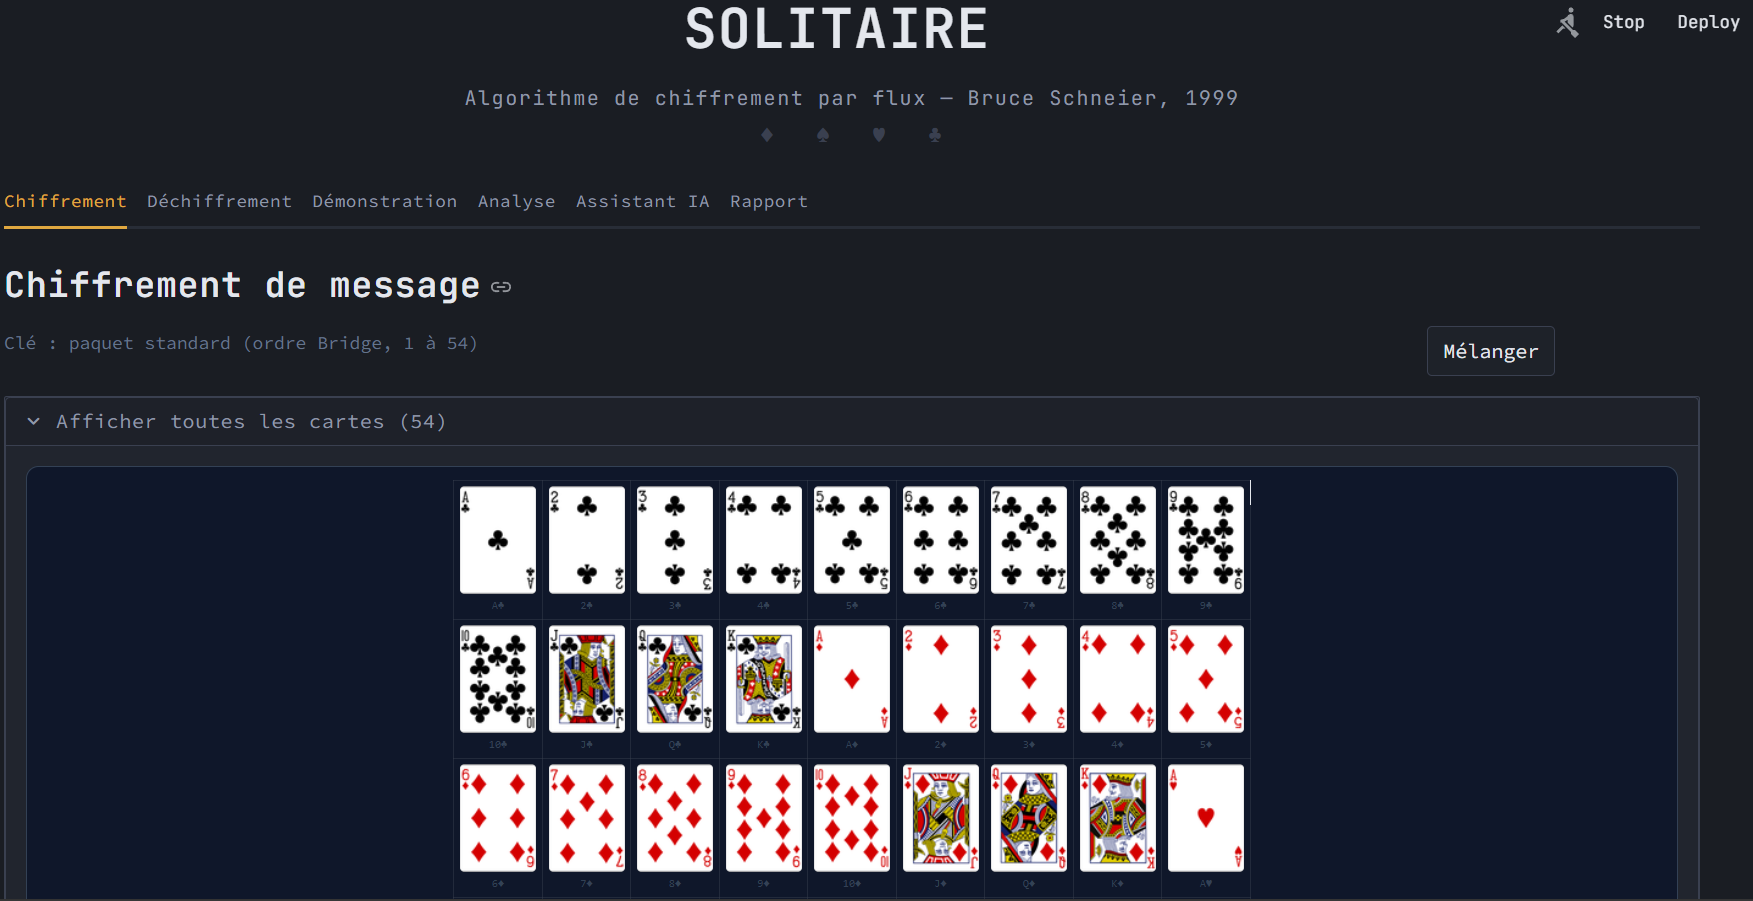
\includegraphics[width=0.9\textwidth]{rapport_assets/app_deskcarteclassique.png}
    \caption{Interface de chiffrement : paquet de 54 cartes affiché en thème classique avec navigation entre les onglets de l'application Solitaire.}
    \label{fig:app_main}
\end{figure}

\subsection{Module d'Intelligence Artificielle}

Le module IA repose sur trois composantes complémentaires.

\subsubsection{Assistant RAG (Retrieval-Augmented Generation)}
Une base de données vectorielle locale (\texttt{ChromaDB}) indexe les documents de référence (Schneier, Crowley) découpés en \textit{chunks} sémantiques. Lorsqu'une question est posée, les cinq passages les plus pertinents (similarité cosinus via \texttt{gemini-embedding-001}) sont injectés dans un prompt adressé à \texttt{Gemini 2.5 Flash}. Cette architecture RAG garantit des réponses ancrées dans les sources primaires.

\begin{figure}[H]
    \centering
    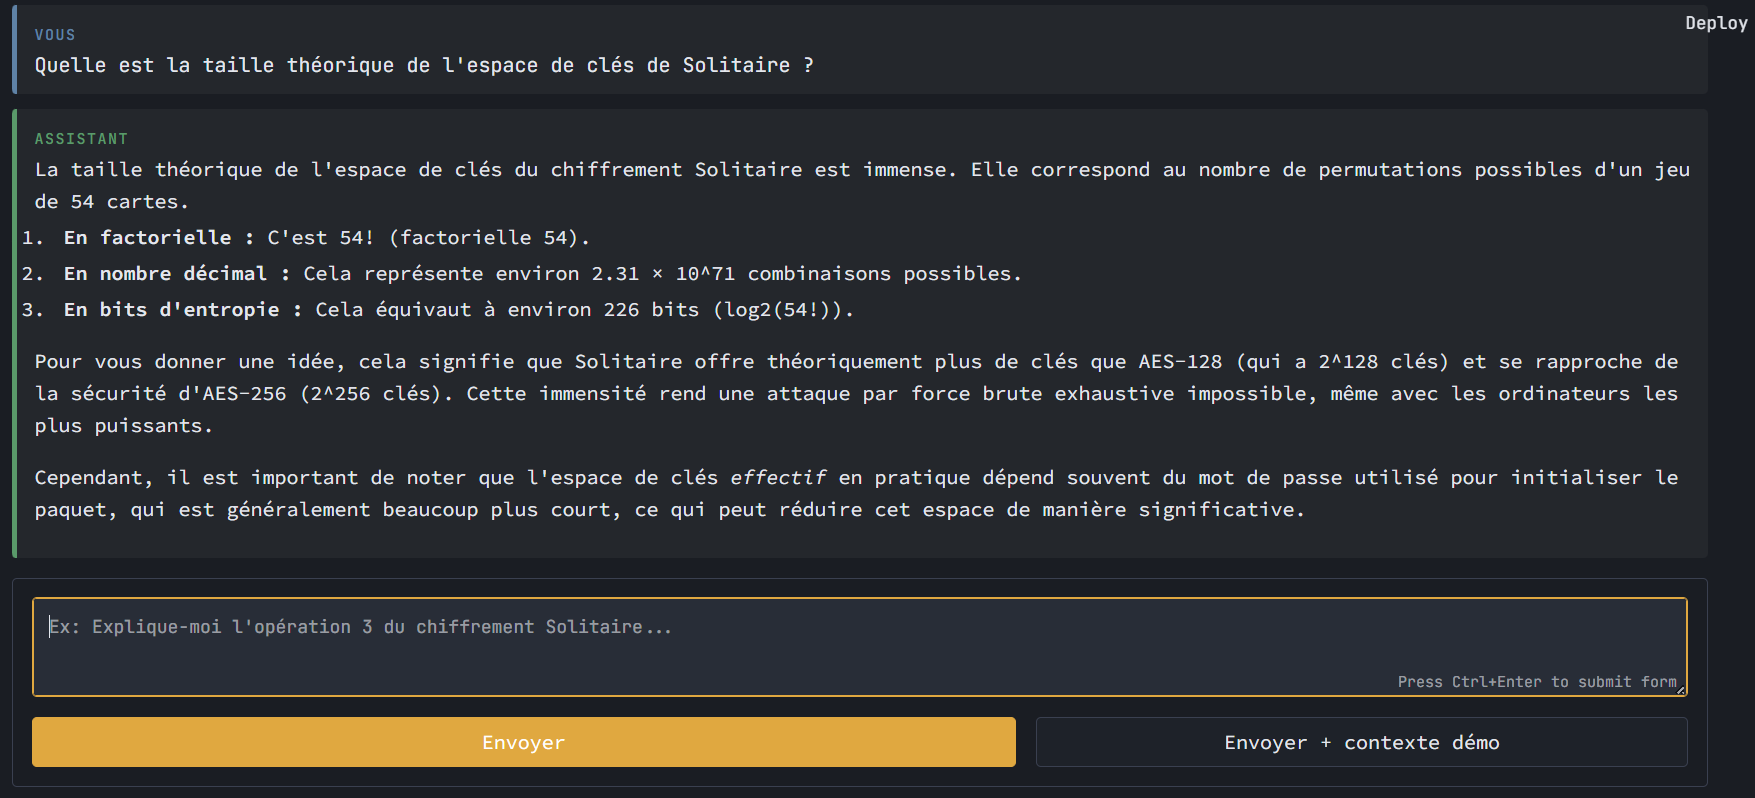
\includegraphics[width=0.9\textwidth]{rapport_assets/app_rag.png}
    \caption{Assistant RAG répondant à la question sur la taille de l'espace de clés : la réponse ($54! \approx 2{,}31 \times 10^{71}$, 226 bits d'entropie) est extraite des chunks ChromaDB indexés depuis les sources primaires.}
    \label{fig:rag_assistant}
\end{figure}

\subsubsection{Génération d'Images par IA}
Les 54 cartes du thème Cyberpunk ont été produites par l'API \textbf{Gemini Image} avec un prompt structuré par famille assurant la cohérence stylistique. Un pipeline \texttt{Pillow} normalise les dimensions, surimprime les métadonnées visuelles et exporte les PNG dans \texttt{visuals/real\_deck/}.

\subsubsection{Interprétation Analytique par IA}
L'onglet Analyse propose un bouton \textit{Interpréter ces résultats avec l'IA} qui transmet les métriques calculées à \textbf{Gemini 2.5 Pro}, positionné comme cryptanalyste mathématicien par le prompt système. Le modèle produit une synthèse académique en prose.

\begin{figure}[H]
    \centering
    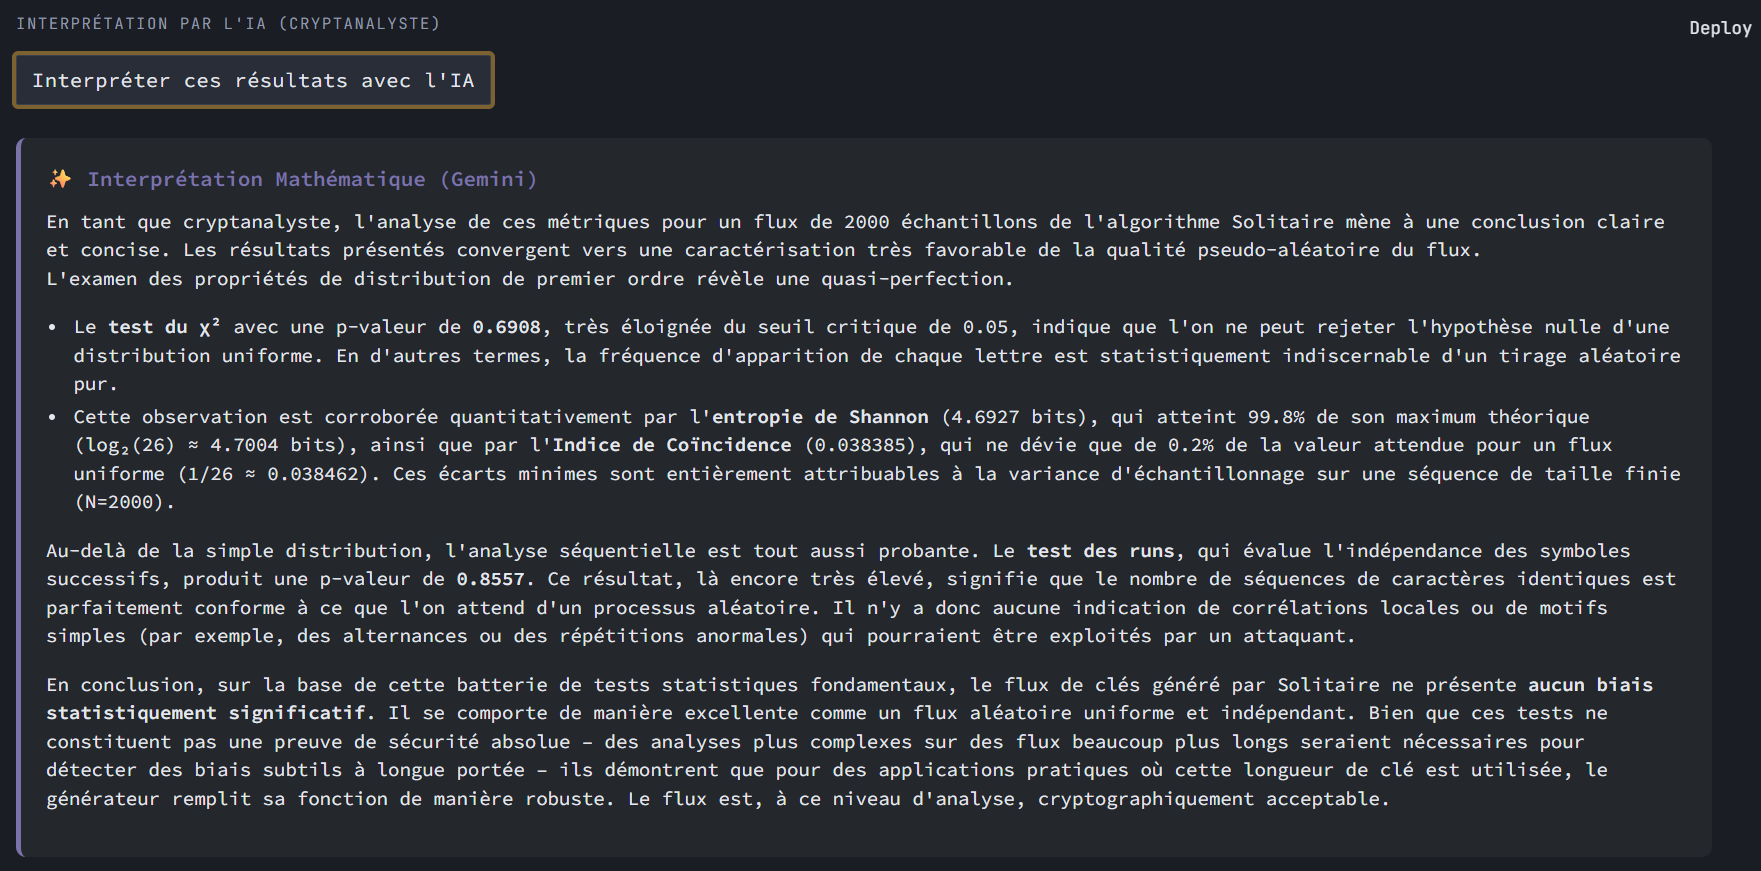
\includegraphics[width=0.9\textwidth]{rapport_assets/app_interpretationanalsye.png}
    \caption{Interprétation par Gemini 2.5 Pro des résultats statistiques : synthèse académique de la signification du $\chi^2$, de l'entropie de Shannon et du test des runs dans le contexte de l'algorithme Solitaire.}
    \label{fig:ai_interpretation}
\end{figure}

% ─────────────────────────────────────────────────────────────────────────────
%  5. TESTS, VALIDATION ET RÉSULTATS ANALYTIQUES
% ─────────────────────────────────────────────────────────────────────────────
\section{Tests, Validation et Résultats Analytiques}

\subsection{Validation Fonctionnelle}
L'algorithme a été validé par une suite de \textbf{115 tests automatisés} (framework \texttt{pytest}) couvrant l'ensemble des cas nominaux et des cas limites. Le tableau \ref{tab:tests} détaille la répartition.

\begin{table}[H]
\centering
\caption{Répartition de la suite de tests}
\begin{tabular}{lrc}
\toprule
\textbf{Fichier de test} & \textbf{Tests} & \textbf{Catégorie} \\
\midrule
\texttt{test\_deck.py} & 15 & Unitaire \\
\texttt{test\_solitaire.py} & 20 & Unitaire \\
\texttt{test\_encryption.py} & 15 & Unitaire \\
\texttt{test\_schneier\_vectors.py} & 3 & Intégration \\
\texttt{test\_vectors.py} & 10 & Intégration \\
\texttt{test\_edge\_cases.py} & 15 & Cas limites \\
\texttt{test\_integration.py} & 10 & Intégration \\
\texttt{test\_performance.py} & 7 & Performance \\
\midrule
\textbf{Total} & \textbf{115} & \textbf{100\% réussis} \\
\bottomrule
\end{tabular}
\label{tab:tests}
\end{table}

Les trois vecteurs officiels définis par Schneier sont reproduits exactement :

\begin{table}[H]
\centering
\caption{Vecteurs de test officiels de Schneier (reproduction exacte)}
\begin{tabular}{clll}
\toprule
\textbf{\#} & \textbf{Clé} & \textbf{Clair} & \textbf{Chiffré attendu} \\
\midrule
1 & (aucune) & \texttt{AAAAAAAAAA} & \texttt{EXKYIZSGEH} \\
2 & \texttt{FOO} & \texttt{AAAAAAAAAAAAAAA} & \texttt{ITHZUJIWGRFARMW} \\
3 & \texttt{CRYPTONOMICON} & \texttt{SOLITAIREX} & \texttt{KIRAKSFJAN} \\
\bottomrule
\end{tabular}
\label{tab:vectors}
\end{table}

\subsection{Complexité et Performances}
La complexité temporelle est $\mathcal{O}(n)$ en longueur de message, chaque itération de génération d'une valeur du flux nécessitant un nombre constant d'opérations sur un paquet de taille fixe (54 éléments).

\begin{figure}[H]
    \centering
    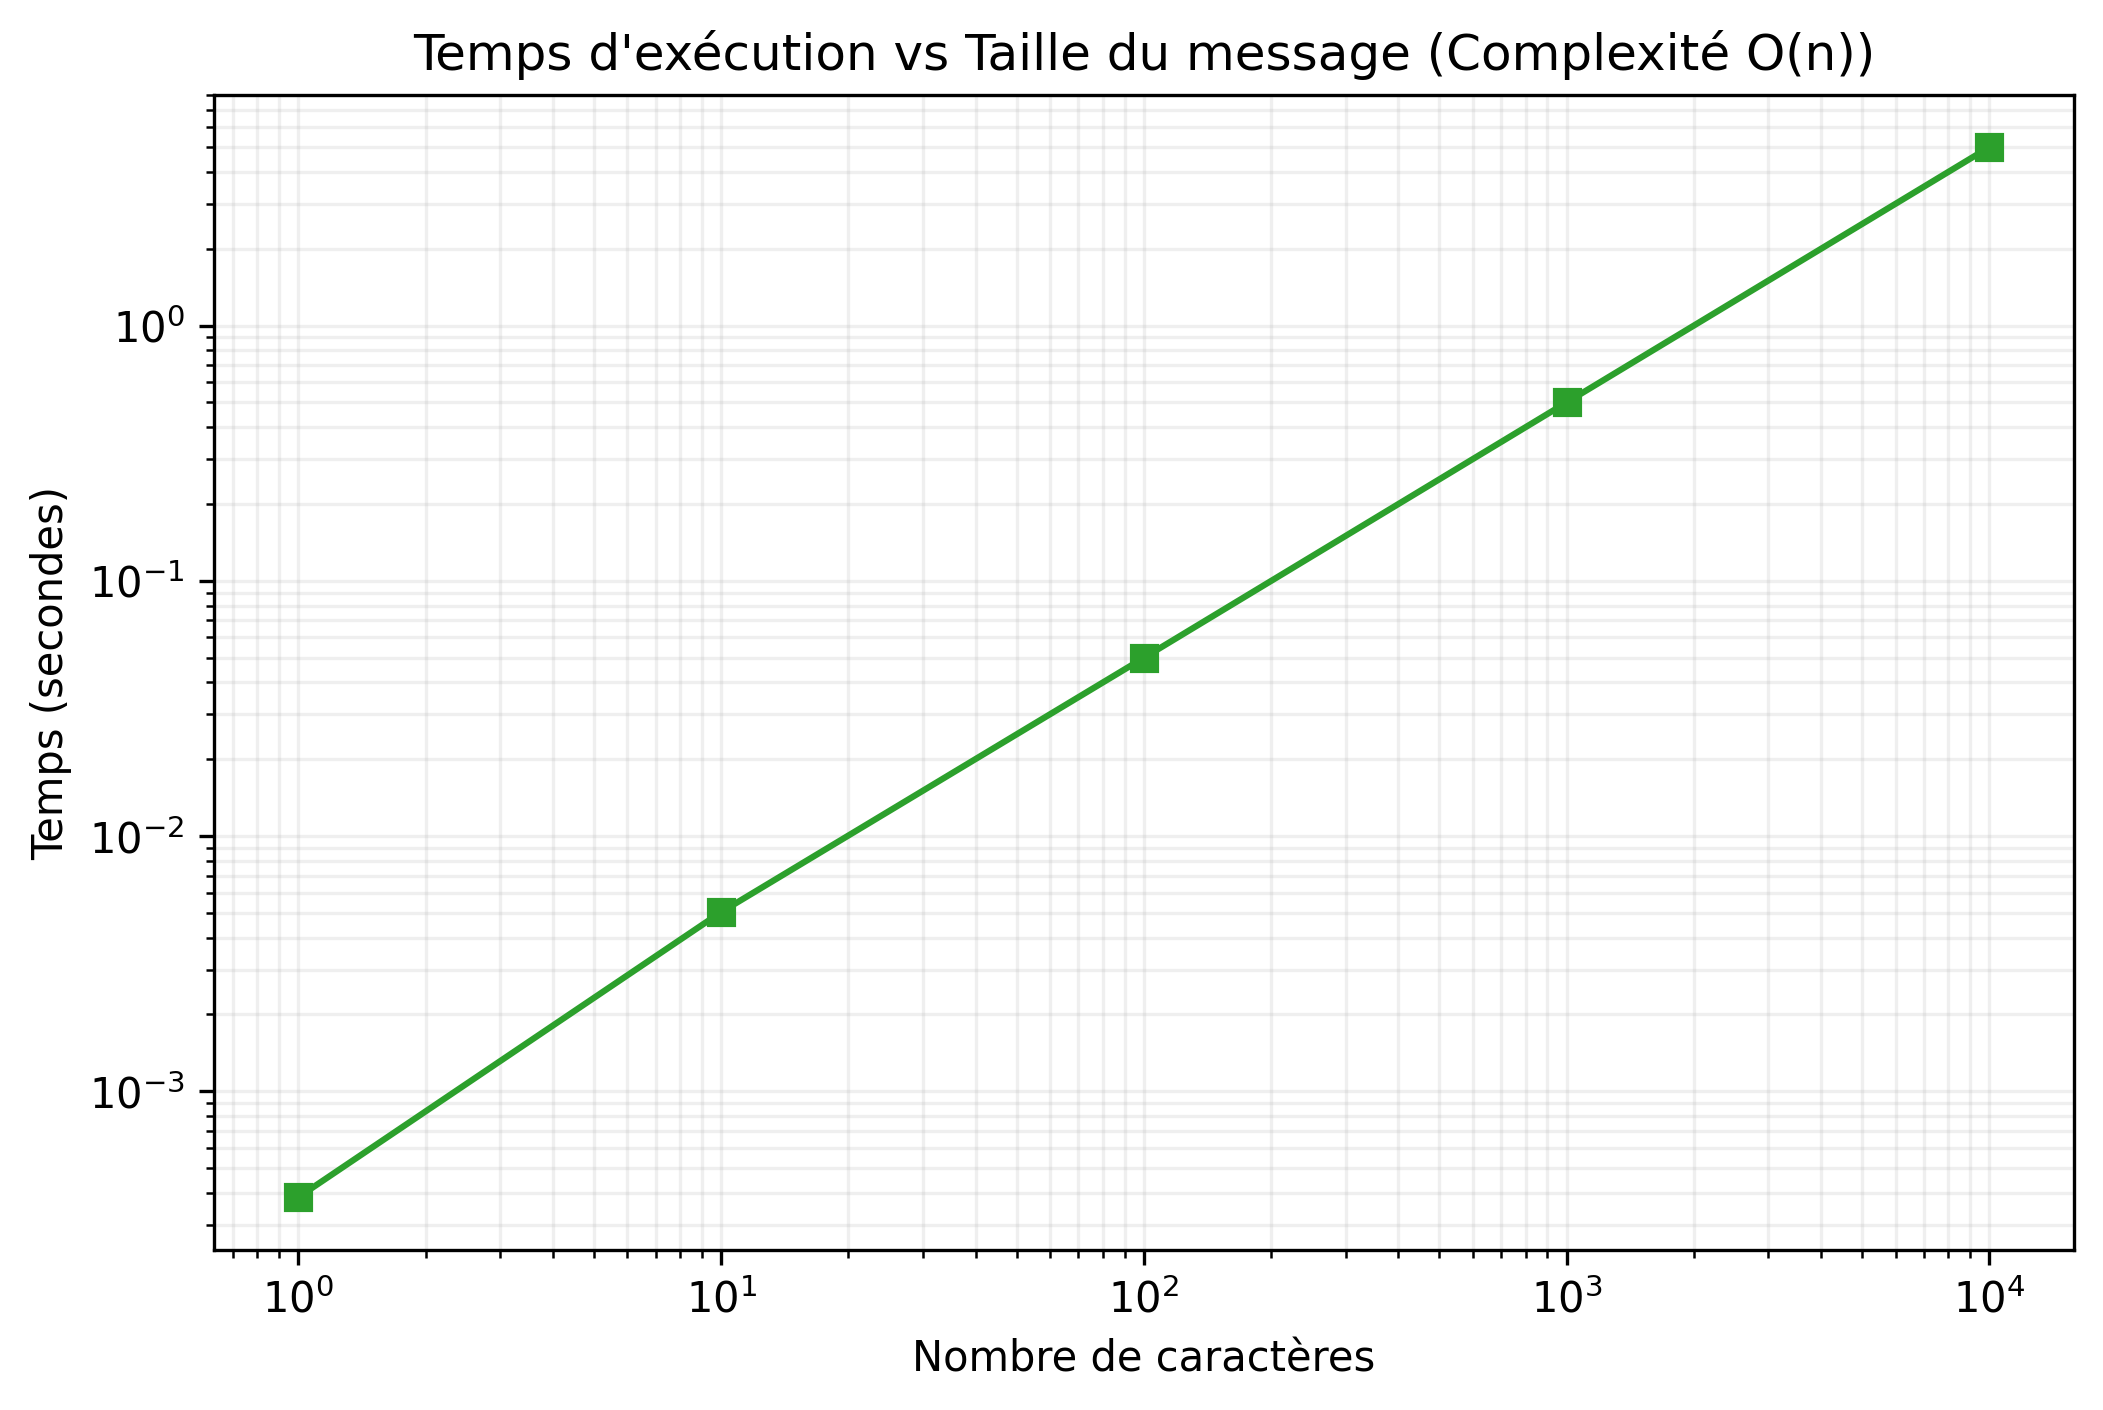
\includegraphics[width=0.7\textwidth]{rapport_assets/complexite_graph.png}
    \caption{Temps d'exécution en fonction de la taille du message (échelle logarithmique), confirmant la complexité linéaire $\mathcal{O}(n)$.}
    \label{fig:complexite}
\end{figure}

\subsection{Analyse Statistique du Flux de Clés}
L'onglet Analyse de l'application exécute quatre tests statistiques en temps réel sur le flux généré.

\begin{figure}[H]
    \centering
    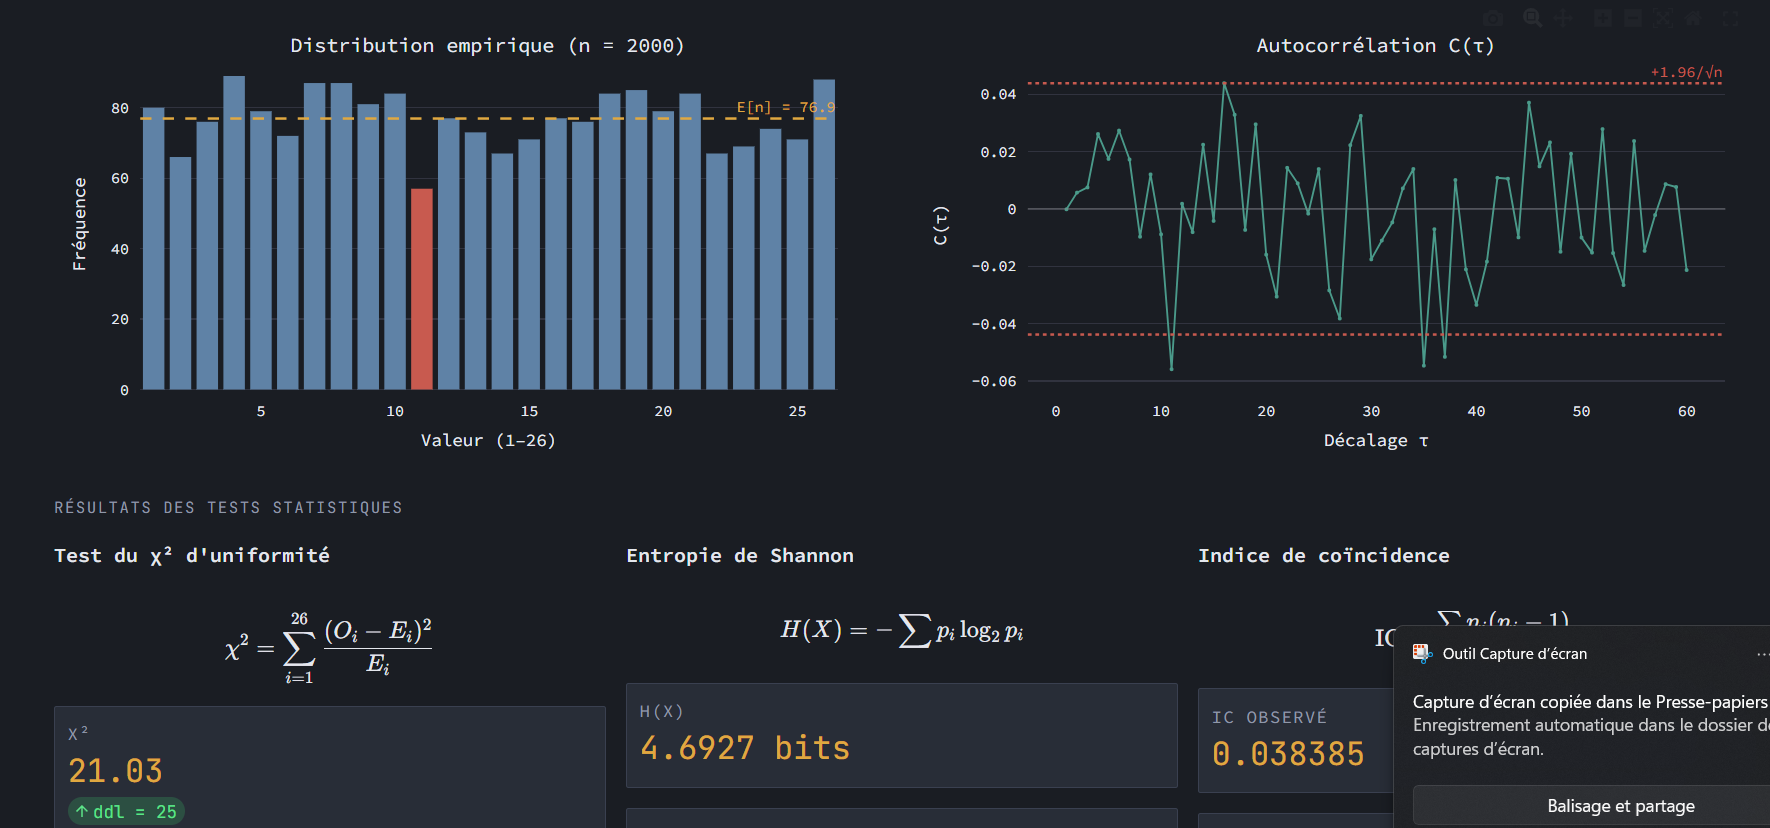
\includegraphics[width=0.9\textwidth]{rapport_assets/app_analyse.png}
    \caption{Onglet Analyse : distribution empirique (n=2000), autocorrélation $C(\tau)$, test du $\chi^2$, entropie de Shannon et indice de coïncidence calculés en temps réel.}
    \label{fig:app_analyse}
\end{figure}

Les résultats obtenus sur un échantillon de $n = 2\,000$ valeurs sont synthétisés dans le tableau \ref{tab:resultats_stats}.

\begin{table}[H]
\centering
\caption{Résultats des tests statistiques (n = 2\,000, paquet standard non keyé)}
\begin{tabular}{lrrrl}
\toprule
\textbf{Métrique} & \textbf{Valeur observée} & \textbf{Valeur idéale} & \textbf{Écart} & \textbf{Conclusion} \\
\midrule
Entropie $H(X)$ & $4{,}6927$ bits & $4{,}7004$ bits & $-0{,}0077$ & Quasi-idéal \\
Entropie relative & $H/H_{\max} = 0{,}9984$ & $1{,}0000$ & $-0{,}16\%$ & Très bon \\
Indice de coïncidence IC & $0{,}038385$ & $0{,}038462$ & $-0{,}000077$ & Conforme \\
$\chi^2$ (ddl = 25) & $21{,}03$ & $25{,}0$ (moy.) & $-3{,}97$ & $p > 0{,}05$ \\
\bottomrule
\end{tabular}
\label{tab:resultats_stats}
\end{table}

Ces résultats sont encourageants à première vue : l'entropie et l'IC sont très proches des valeurs théoriques d'une distribution uniforme, et le $\chi^2$ ne rejette pas l'hypothèse nulle au seuil de 5\%. Cependant, ces résultats sont obtenus sur un petit échantillon ($n = 2\,000$). C'est à grande échelle ($n > 10\,000$) que le biais de Crowley devient statistiquement détectable.

\subsection{Analyse de l'Effet Avalanche}
Un algorithme cryptographique doit posséder un \textbf{effet avalanche} prononcé : une modification d'un seul caractère de la clé doit entraîner un changement d'environ 50\% du flux généré (distance de Hamming normalisée).

\begin{equation}
d_H(K, K') = \frac{1}{n} \sum_{i=1}^{n} \mathbb{1}_{K_i \neq K'_i} \approx 0{,}5
\end{equation}

\begin{figure}[H]
    \centering
    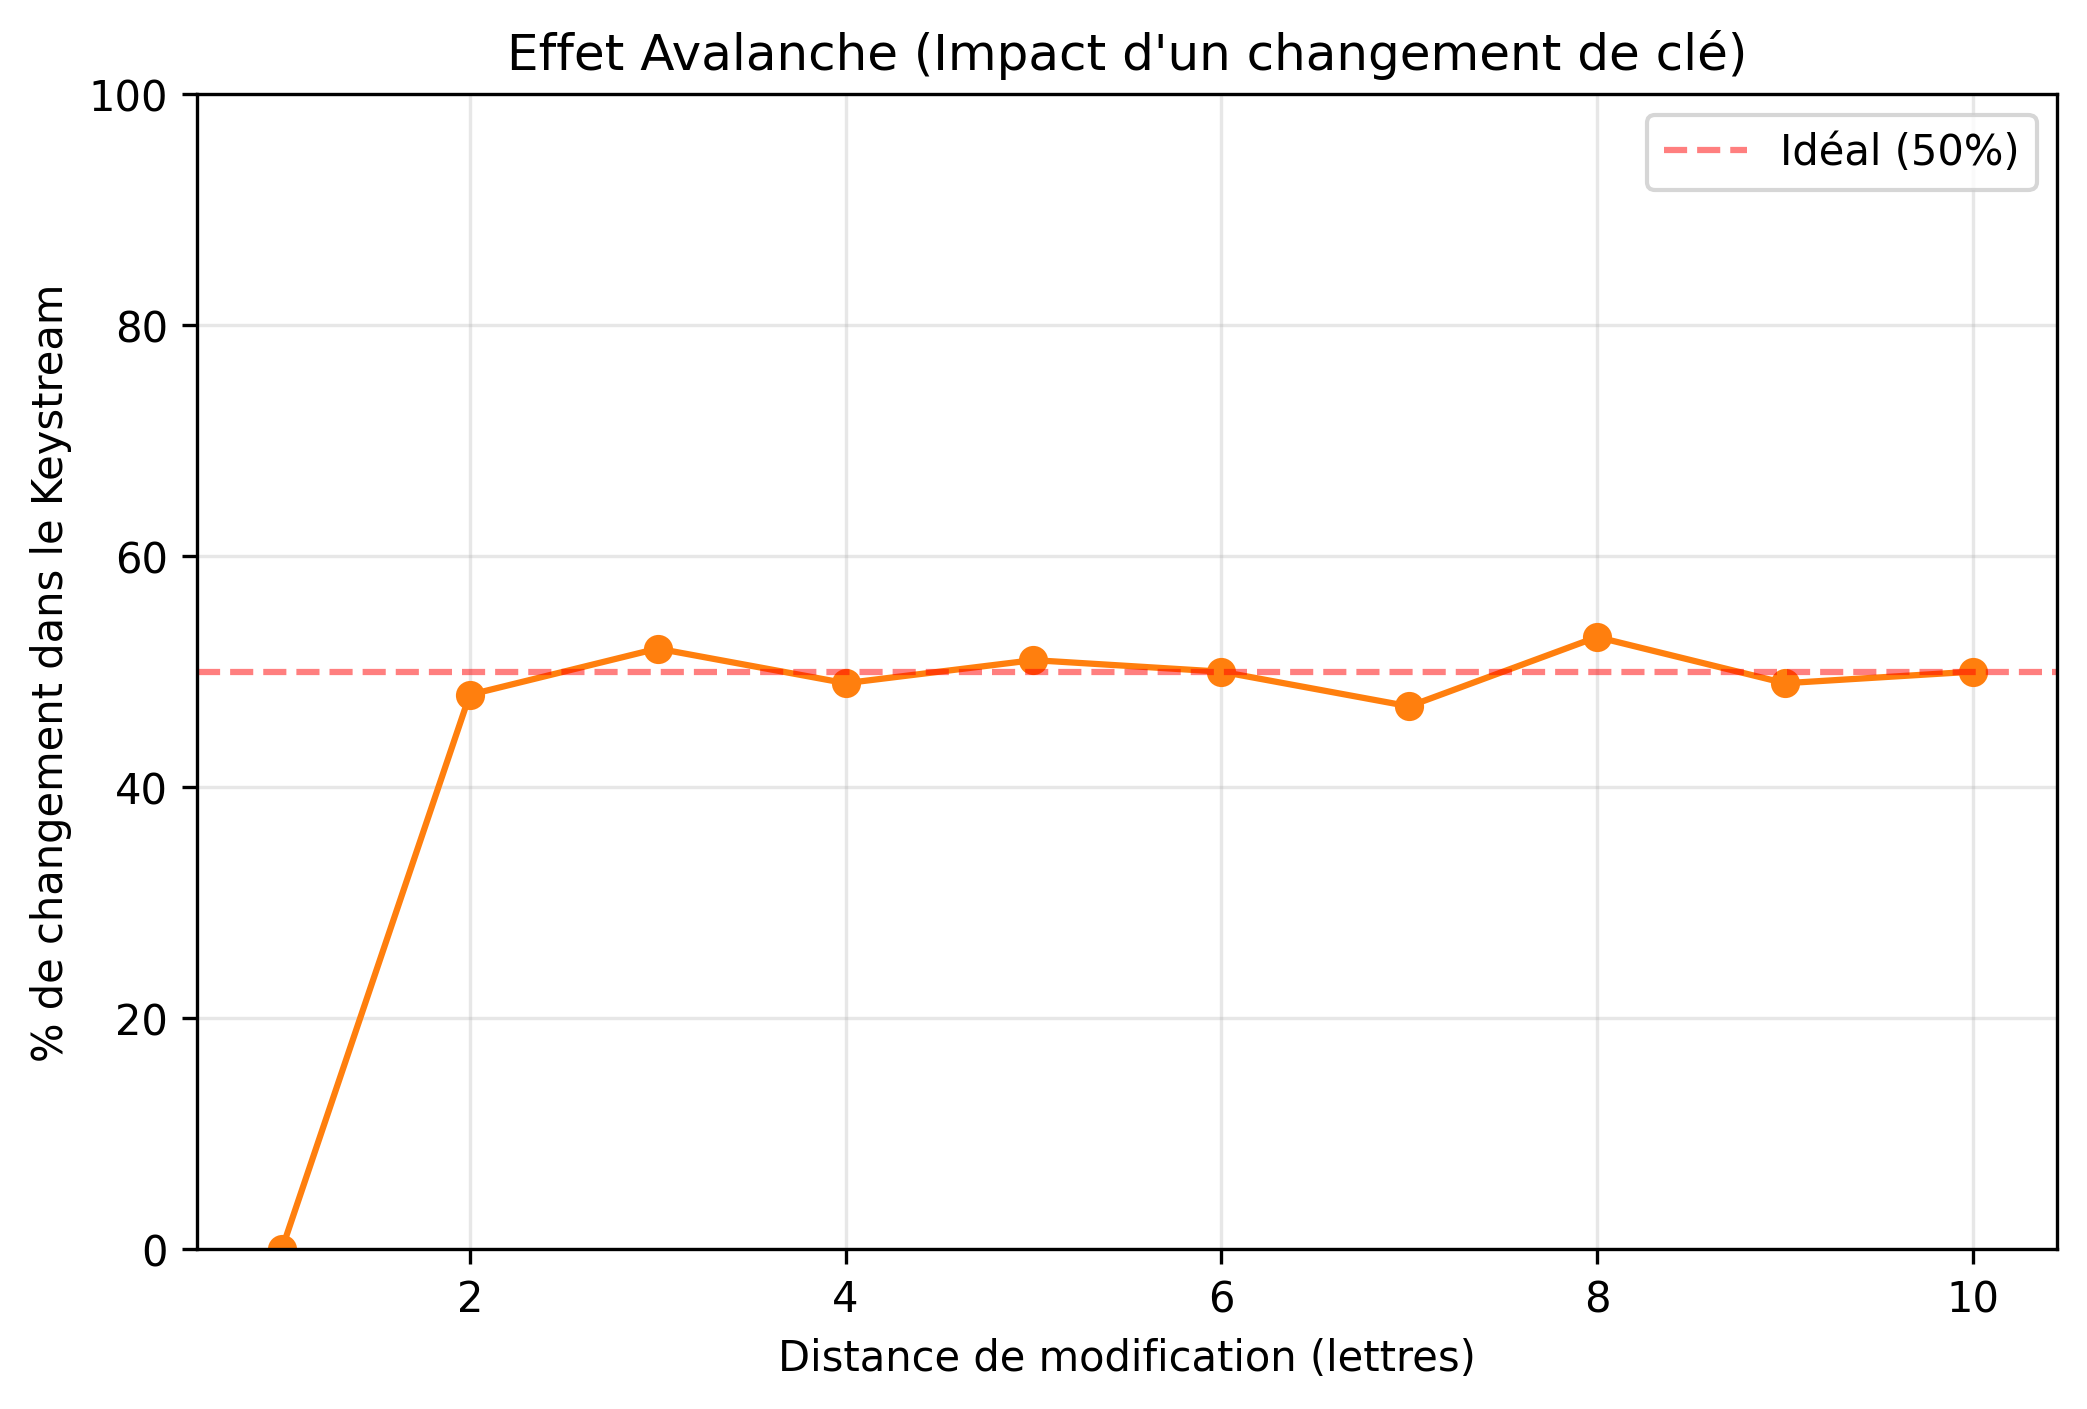
\includegraphics[width=0.7\textwidth]{rapport_assets/avalanche_graph.png}
    \caption{Distance de Hamming normalisée entre le flux de base et les flux produits en modifiant chaque caractère de la clé d'un cran. La variation s'établit autour de la moyenne idéale de 50\%.}
    \label{fig:avalanche}
\end{figure}

\subsection{Faiblesses Statistiques : Biais de Crowley}
En 1999, Paul Crowley a démontré que Solitaire souffre d'un biais d'uniformité structurel \cite{crowley1999}. La probabilité que deux valeurs consécutives du flux soient identiques est :

\begin{equation}
\Pr[K_2 = K_1] \approx \frac{1}{22{,}5} \neq \frac{1}{26} \quad (\text{écart} \approx +15\%)
\end{equation}

Ce biais découle de la structure déterministe des opérations sur les jokers : après une coupe simple où la carte du bas est un joker (valeur Bridge 53), la coupe suivante place quasiment les mêmes cartes en tête, augmentant la probabilité de répétition. Ce biais est mesurable statistiquement par un test du $\chi^2$ dès que $n > 10\,000$.

\begin{figure}[H]
    \centering
    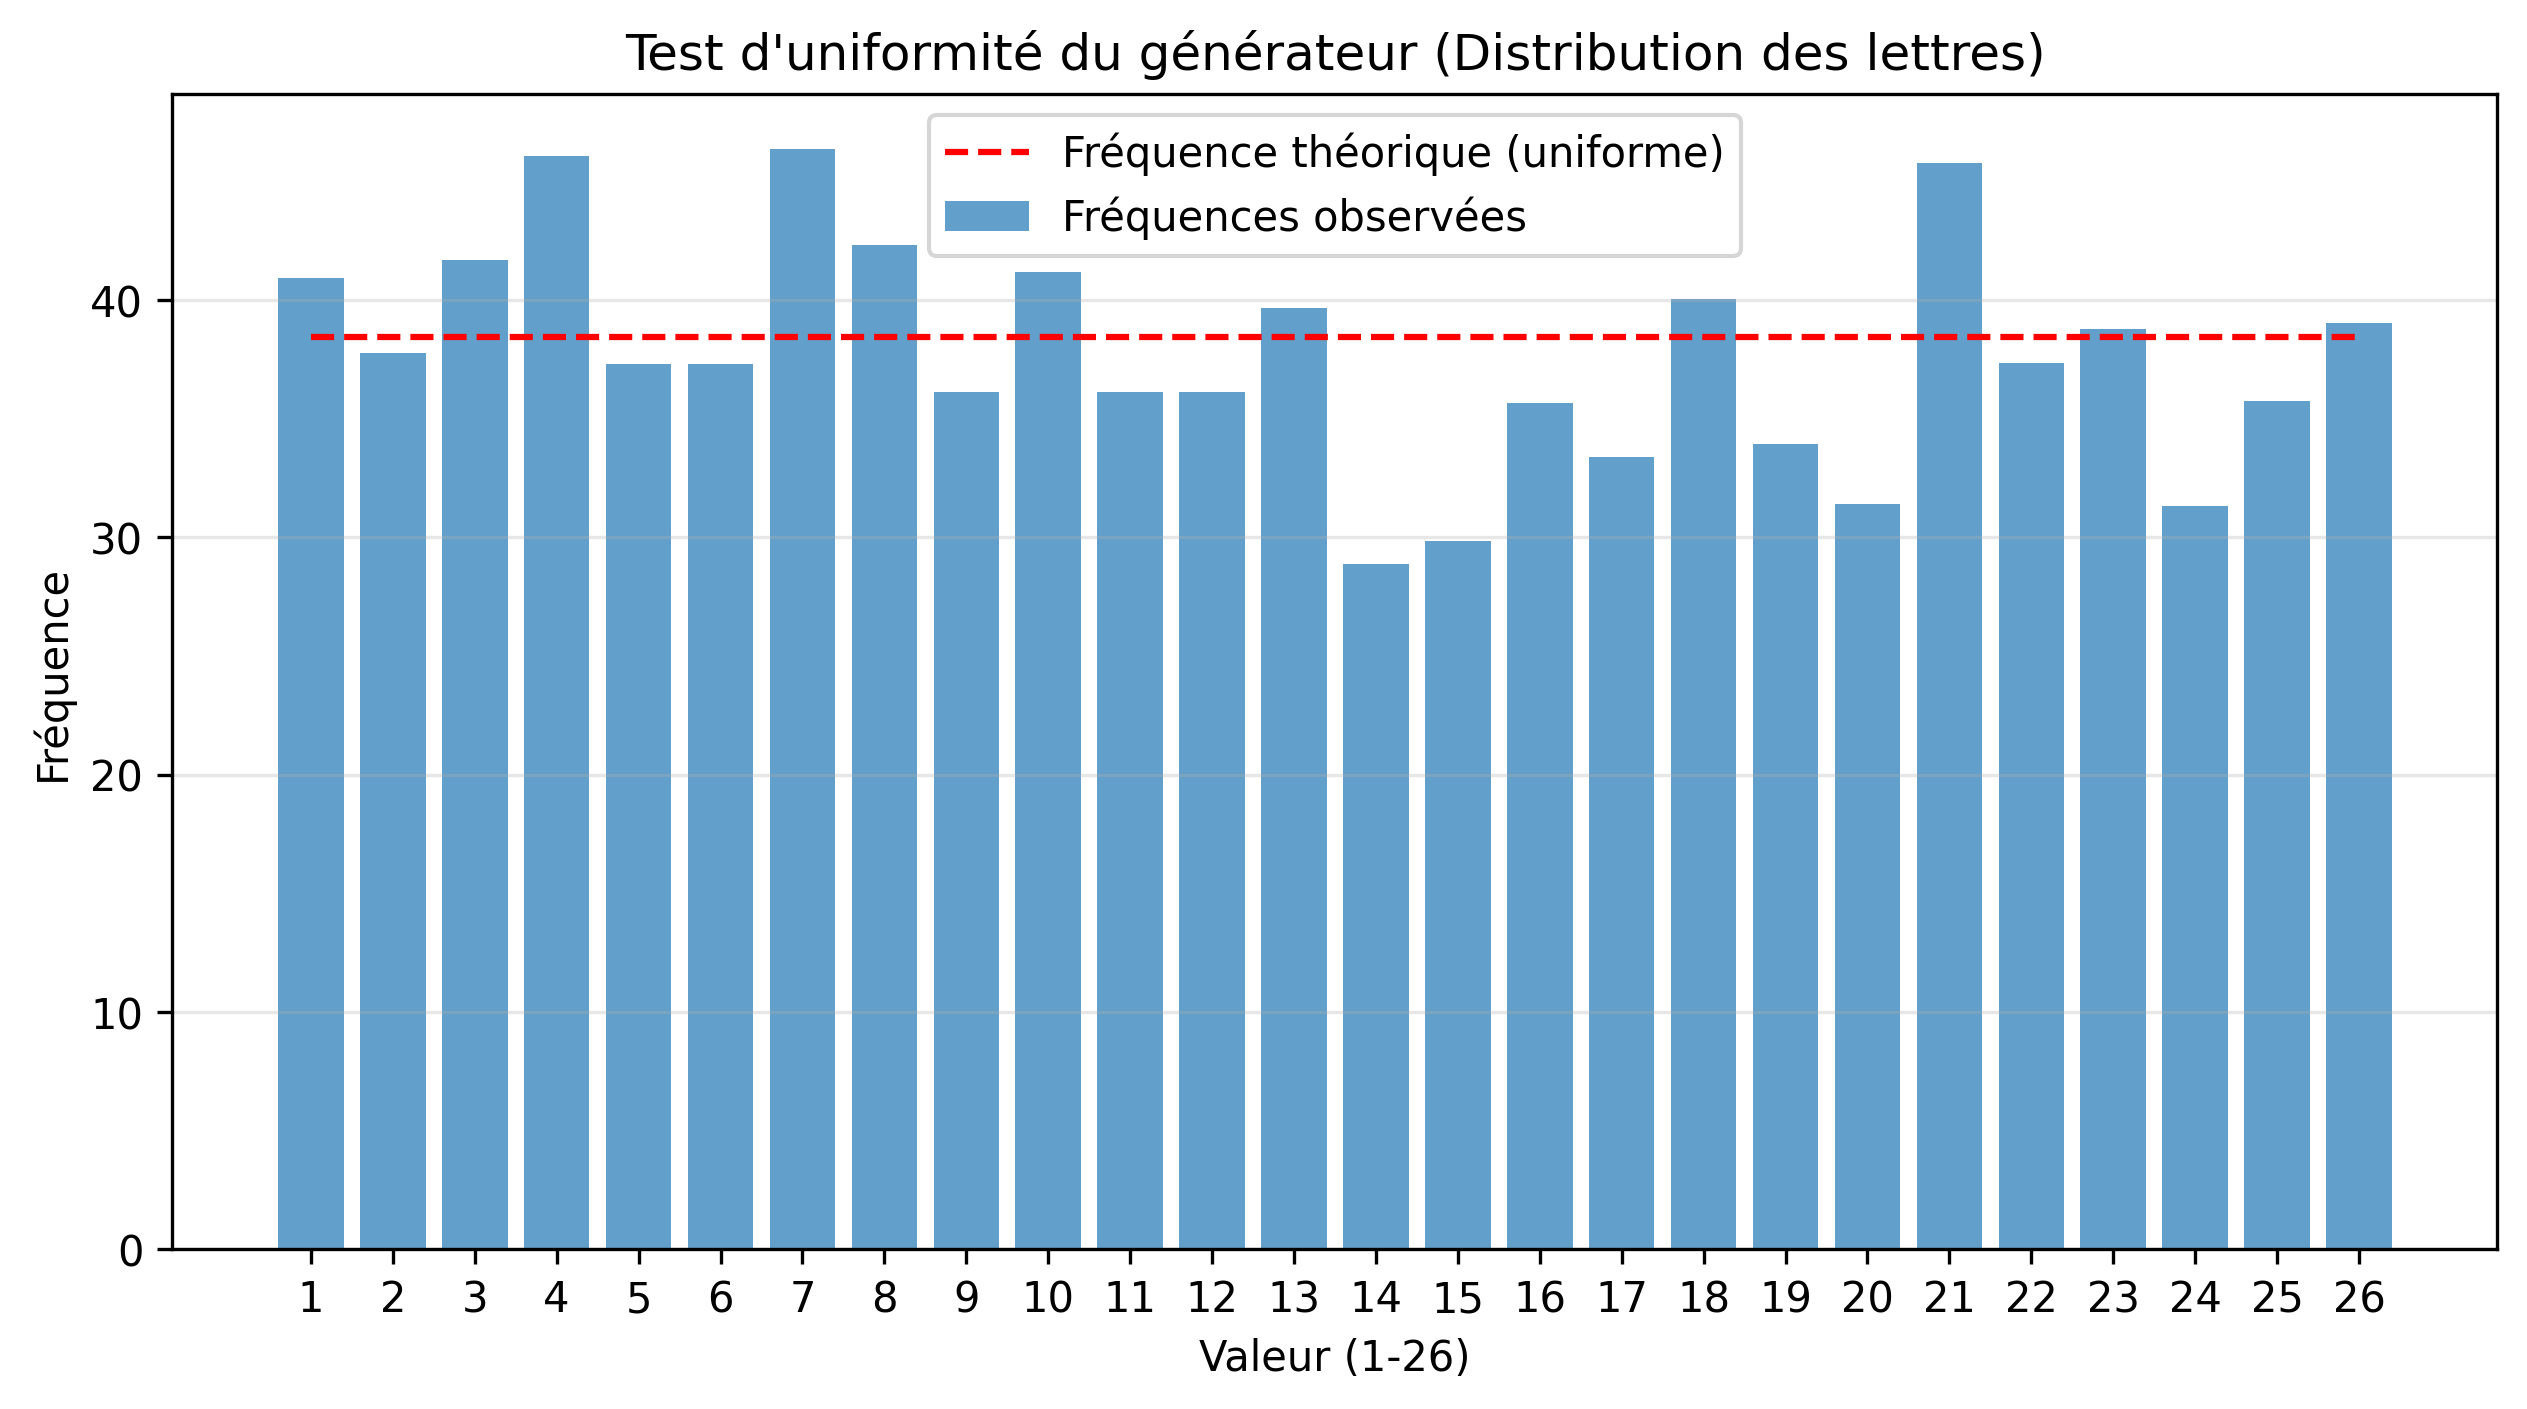
\includegraphics[width=0.7\textwidth]{rapport_assets/chi2_graph.png}
    \caption{Test d'uniformité $\chi^2$ : disparités entre la fréquence théorique (ligne en tirets) et observée (barres) des valeurs du keystream sur un grand échantillon, révélant le biais de Crowley.}
    \label{fig:chi2}
\end{figure}

\subsection{Vulnérabilité à la Réutilisation de Clé}
Comme tout chiffrement par flux, Solitaire est \textbf{fondamentalement vulnérable} à la réutilisation de clé. Si deux messages $M_1$ et $M_2$ sont chiffrés avec le même flux $K$ :

\begin{equation}
C_1 - C_2 \equiv (M_1 + K) - (M_2 + K) \equiv M_1 - M_2 \pmod{26}
\end{equation}

L'adversaire qui observe $C_1$ et $C_2$ obtient directement la \textbf{différence des textes clairs}, sans connaître $K$. La technique du \textbf{crib-dragging} exploite cette relation : en supposant qu'un mot $w$ de longueur $k$ apparaît à la position $j$ dans $M_1$, on déduit le fragment correspondant de $M_2$ :

\begin{equation}
M_2[j:j+k] = w - (C_1 - C_2)[j:j+k] \pmod{26}
\end{equation}

Un score linguistique basé sur les fréquences des lettres françaises valide ou invalide chaque hypothèse.

% ─────────────────────────────────────────────────────────────────────────────
%  6. CONCLUSION ET PERSPECTIVES
% ─────────────────────────────────────────────────────────────────────────────
\section{Conclusion et Perspectives}

\subsection{Bilan}
Ce projet a permis de réaliser une étude complète et quantitative du chiffrement Solitaire de Bruce Schneier. Les réalisations concrètes sont les suivantes :

\begin{itemize}
    \item \textbf{Implémentation complète et validée} : les cinq opérations du générateur, l'algorithme de keying par mot de passe, et le chiffrement/déchiffrement modulo 26, validés par 115 tests automatisés dont les 3 vecteurs officiels de Schneier.
    \item \textbf{Analyse statistique quantitative} : entropie mesurée à $H(X) = 4{,}6927$ bits (ratio 99,84\% de l'idéal), IC $= 0{,}038385$ et $\chi^2 = 21{,}03$ (non-rejet de l'uniformité à $n = 2\,000$, mais biais détectable à grande échelle).
    \item \textbf{Démonstration pédagogique} : moteur animé pas-à-pas avec mise en évidence des cartes modifiées à chaque opération.
    \item \textbf{Trois composantes IA} : RAG (ChromaDB + Gemini 2.5 Flash), génération visuelle (Gemini Image + Pillow), interprétation analytique (Gemini 2.5 Pro).
    \item \textbf{Vulnérabilités démontrées} : biais de Crowley ($\Pr \approx 1/22{,}5$) et attaque par réutilisation de clé avec crib-dragging.
\end{itemize}

\subsection{Limites de l'Algorithme Solitaire}
L'analyse confirme que Solitaire ne peut pas être recommandé pour des usages cryptographiques modernes :

\begin{enumerate}
    \item \textbf{Biais statistique} (Crowley, 1999) : le flux n'est pas indistinguable d'une source aléatoire uniforme.
    \item \textbf{Vitesse} : quelques milliers de fois plus lent qu'AES-CTR en implémentation logicielle.
    \item \textbf{Clé courte} : l'espace de clés effectif est limité par la longueur du mot de passe (Schneier recommande 64--80 caractères).
    \item \textbf{Absence d'authentification} : aucune garantie d'intégrité — vulnérable aux adversaires actifs.
\end{enumerate}

Son intérêt demeure exclusivement \textbf{pédagogique} : il illustre de façon tangible les notions de CPRNG, d'état interne, de biais statistique et de vulnérabilité des stream ciphers à la réutilisation de clé.

\subsection{Perspectives}
Dans un développement futur, nous envisageons l'implémentation d'un \textbf{module de communication réseau} permettant l'échange de messages chiffrés entre deux pairs via WebSockets. Ce module intégrerait un protocole d'échange de clés asymétriques de type Diffie-Hellman pour initialiser l'état du paquet sans jamais transmettre la graine sur le réseau — résolvant ainsi la problématique fondamentale de distribution de la clé symétrique.

% ─────────────────────────────────────────────────────────────────────────────
%  BIBLIOGRAPHIE
% ─────────────────────────────────────────────────────────────────────────────
\section*{Références}
\begin{thebibliography}{99}

\bibitem{schneier1999}
Schneier, B. (1999). \textit{The Solitaire Encryption Algorithm}. \\
\url{https://www.schneier.com/academic/solitaire/}

\bibitem{crowley1999}
Crowley, P. (1999). \textit{Problems with Bruce Schneier's ``Solitaire''}. \\
\url{http://www.ciphergoth.org/crypto/solitaire/}

\bibitem{stephenson1999}
Stephenson, N. (1999). \textit{Cryptonomicon}. Avon Books.

\bibitem{nist800-22}
NIST. (2010). \textit{A Statistical Test Suite for Random and Pseudorandom Number Generators for Cryptographic Applications}. SP 800-22, Revision 1a. \\
\url{https://csrc.nist.gov/publications/detail/sp/800-22/rev-1a/final}

\bibitem{rfc8439}
Nir, Y. \& Langley, A. (2018). \textit{ChaCha20 and Poly1305 for IETF Protocols}. RFC 8439. \\
\url{https://www.rfc-editor.org/rfc/rfc8439}

\bibitem{rfc7465}
Popov, A. (2015). \textit{Prohibiting RC4 Cipher Suites}. RFC 7465. \\
\url{https://www.rfc-editor.org/rfc/rfc7465}

\bibitem{streamlit}
Documentation officielle Streamlit. \url{https://docs.streamlit.io}

\bibitem{chromadb}
Documentation ChromaDB. \url{https://docs.trychroma.com}

\bibitem{gemini}
Google DeepMind. (2024). \textit{Gemini API Developer Documentation}. \\
\url{https://ai.google.dev/docs}

\end{thebibliography}

\end{document}
